\section{Method}
\label{sec:prelim}
\begin{figure*}[t]
    \centering
    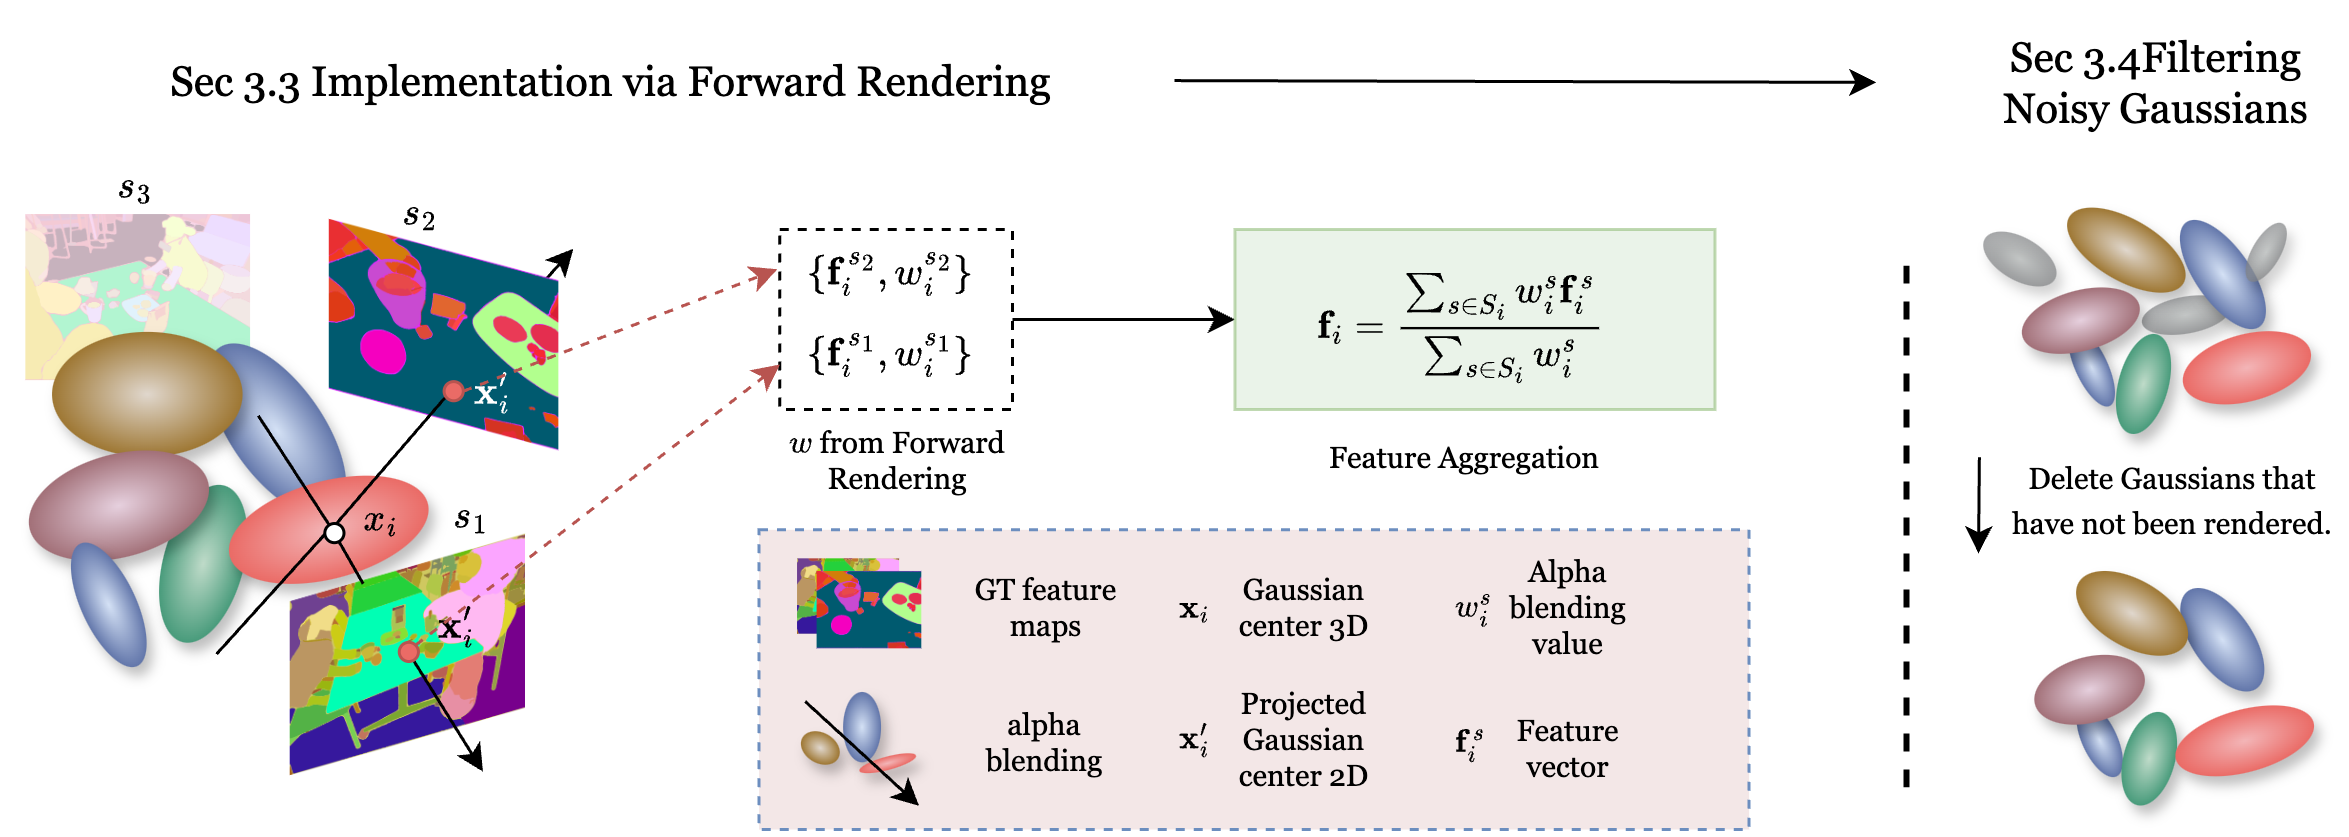
\includegraphics[width=0.8\textwidth, trim={20 0 20 0}, clip]{figures/overview2.png}
    \caption{Overview of our method: Occam's LGS consists of two main stages: (1) Forward rendering process of 3D Gaussian Splatting to obtain alpha blending weights $w$, projected positions $x_i'$ for each Gaussian and their corresponding pixels $p_i$ in 2D views, followed by weighted aggregation of multi-view semantic features (Sec. 3.3); and (2) Filtering of noisy Gaussians that remain invisible throughout the rendering process (Sec. 3.4).}
    \label{fig:overview}
\end{figure*}

The following section provides an overview of our method, which establishes a theoretically grounded and efficient approach for uplifting 2D features to 3D space. It introduces the background on Gaussian splatting rendering, our formulation of maximum likelihood features uplifting, and its implementation via forward rendering and postprocessing by filtering. An overview of the flow of our method is visually presented in Figure~\ref{fig:overview} and further detailed in Algorithm~\ref{alg:algorithm1}.

\subsection{Gaussian Splatting Rendering}
3D Gaussian Splatting represents a scene as a collection of anisotropic Gaussians, where each Gaussian is defined by its position \(\mathbf{x} \in \mathbb{R}^3\), covariance \(\Sigma \in \mathbb{R}^6\), color represented by either a 3D color representation \(\mathbf{c} \in \mathbb{R}^3\), or a viewpoint dependent representation as spherical harmonics~(SH) parameters, and opacity \(o \in \mathbb{R}\)
\begin{equation}
    G(\mathbf x) = e^{-\frac{1}{2}(\mathbf{x})^{\intercal}\Sigma^{-1}(\mathbf{x})}.
\end{equation}
The primitive representation of a Gaussian is defined as $G = \{\mathbf{x}, \Sigma, \mathbf{c}, o\}$, and let $\mathcal{G}=\{G_i\}_{i=1}^N$ be the set of Gaussians in a scene. For rendering, we first project each 3D Gaussian onto the image plane, resulting in a 2D Gaussian $G' = \{\mathbf{x'}, \Sigma', \mathbf{c}, o\}$, with $\mathbf{x'} \in \mathbb{R}^2$ as the projected 2D coordinates and $\mathbf{\Sigma'} \in \mathbb{R}^{2\times2}$ as the projected covariance matrix.

To render the color at pixel $\mathbf{p}$, we blend the contributions of all Gaussians along the ray originating from the camera center, say $\mathcal{G}^r = \{G_k\}_{k=1}^R$, where $R$ is the total number of Gaussians along the ray. To achieve efficient rendering in the Gaussian Splatting framework, this rendering process is implemented through a tile-based sorting strategy, which utilizes the approximation of Gaussians by a spatially truncated distribution. For this purpose, the image is partitioned into tiles, typically spanning 16x16 pixels. Each 2D Gaussian is assigned to all tiles intersecting with a bounding box placed at the 3$\sigma$ boundary. Within each tile, Gaussians are sorted by depth from the camera center. These sorted Gaussians represent the collection of Gaussians that potentially contribute to any pixel within that tile, which are then rendered sequentially, starting closest to the camera. The tiling approach implements an efficient ray-Gaussian intersection test: if a Gaussian's bounding box intersects a tile, it is a candidate to contribute to the rays passing through that tile's pixels.

For the \(i\)-th Gaussian in the sorted list, its contribution to a pixel $\mathbf{p}$ is defined as $\alpha_i = o_i G_i(\mathbf{x}_i')$, representing its influence. When projecting all relevant Gaussians, the color of the pixel $\mathbf{p}$ is computed through a weighted blending process given by
\begin{equation}
 \mathcal{C}(\mathbf{p}) = \psi_c (\mathbf{p}, \mathcal{G}) = \sum_{i=1}^{R} \alpha_i \mathbf{c}_i \prod_{j=1}^{i-1} (1 - \alpha_j),
 \label{eq:colorR}
\end{equation}
where, $\psi_c(,.,)$ is the color rendering function. Specifically, the contribution of $G_i$ to pixel $\mathbf{p}$ is computed as
\begin{equation}
    \alpha_i = \mathbf{o}_i \cdot e^{-\frac{1}{2}((\mathbf{p} - \mathbf x_i ')^{\intercal}\Sigma^{-1}(\mathbf{p} - \mathbf x_i ')}.
    \label{eq:featureR}
\end{equation}


With the goal of lifting multi-view 2D features into 3D space, we extend each Gaussian representation to include a high-dimensional semantic feature vector $\mathbf{f} \in \mathbb{R}^{d}$. Thus, each augmented 3D Gaussian $G_i$ learns its own semantic feature $\mathbf{f_i}$. Similar to color blending, the semantic feature at pixel $\mathbf{p}$ is computed through alpha-weighted blending
\begin{align}
\mathcal{F}(\mathbf{p}) = \psi_f (\mathbf{p}, \mathcal{G}) & = \sum_{i=1}^{R} \alpha_i \mathbf{f}_i\prod_{j=1}^{i-1} (1 - \alpha_j) \\
&= \sum_{i=1}^{R} w_i \mathbf{f}_i  
\label{eq:featureR}
\end{align}
where $\psi_f$ is the feature rendering function and $w_i = \alpha_i\prod_{j=1}^{i-1} (1 - \alpha_j)$ represents the alpha blending weight for Gaussian $i$. 

It is important to note that explicit rendering of semantics according to Equation~\eqref{eq:featureR} is expensive both in memory and computation when compared to the rendering of color in Equation~\eqref{eq:colorR}. This is due to the considerably higher dimensionality of the features $d>>3$, which prevents the GPU from fitting all required data in the shader L1 cache~\cite{qin2024langsplat}.

\subsection{Maximum Likelihood Feature Uplifting}
We deeply ground our approach to feature uplifting in the principles of 3DGS and probabilistic modeling. While conventional semantic feature learning methods~\cite{wu2024opengaussian, guo2024semantic} rely on back-projection, where 2D pixel-space language features are projected back to 3D space through ray-tracing, we leverage the underlying mathematical structure of Gaussian Splatting's forward rendering process to establish a more precise and theoretically sound feature lifting mechanism and relate it to forward modeling.

We formulate the feature uplifting problem as a Maximum-a-Posteriori (MAP) estimation problem. Given 2D feature maps $\mathbf{F}^{2D}$, the MAP estimator of 3D features $\mathbf{f}$ is:
\begin{equation}
\arg\max_\mathbf{f} p(\mathbf{f}|\mathbf{F}^{2D}) = \arg\max_\mathbf{f} p(\mathbf{F}^{2D}|\mathbf{f})\frac{p(\mathbf{f})}{p(\mathbf{F}^{2D})}
\end{equation}
For language gaussian splatting with uniformly distributed language features $p(\mathbf{f})$, which we assume for the efficient feature space of CLIP, the estimator simplifies to the Maximum Likelihood (ML) formulation $\arg\max_\mathbf{f} p(\mathbf{F}^{2D}|\mathbf{f})$.

Under a Gaussian noise model $\epsilon_{p,v}$ for language features and conditional independence of pixels, the rendered 2D feature at pixel $p$ in view $v$ is $\mathbf{f}_{p,v}^{2D} = \sum_{k=1}^R w_{k,p,v}\mathbf{f}_k + \epsilon_{p,v}$. This leads to the weighted aggregation formula for the 3D feature of each Gaussian
\begin{equation}
\boxed{
\mathbf{f}_i = \frac{\sum\limits_{s \in S_i} w_i^s \mathbf{f}_i^s}{\sum\limits_{s \in S_i} w_i^s}
}
\label{eq:wtd.agg}
\end{equation}
where $S_i$ is the set of views where Gaussian $i$ is visible, $w_i^s$ represents the contribution (alpha blending weight) of Gaussian $i$ at its center projection in view $s$, and $\mathbf{f}_i^s$ is the 2D feature at Gaussian $i$'s center projected pixel in view s.
This formula emerges naturally from our probabilistic framework and provides a solution that weights each view's contribution according to the Gaussian's influence in that view. Views, where a Gaussian is more prominent (with a higher alpha blending weight), contribute more significantly to its 3D feature, addressing the challenge of noisy or partially occluded perspectives. We provide complete step-by-step derivation in the supplementary material.


\subsection{Implementation via Forward Rendering}
Our weighted aggregation formula directly maps to the forward rendering process, enabling an efficient implementation that avoids complex back-projection or iterative optimization.
Given a trained visual Gaussian model, for each Gaussian $G_i$ we perform the following steps:
\begin{enumerate}
    \item Identify the set of views $S_i$ where the Gaussian $G_i$ is visible (within the view frustum).
    \item Determine the Gaussian's center projected pixel location $\mathbf{p}_i^s = \lfloor\mathbf{x}_i'\rfloor$ in each view $s$.
    \item Record the alpha blending weight $w_i^s$ and extract the 2D feature $\mathbf{f}_i^s$ at each center projected pixel.
    \item Compute the weighted average following Equation~\ref{eq:wtd.agg}.
\end{enumerate}
This implementation leverages the existing tile-based rendering architecture, allowing us to record projection locations and alpha values during the optimized standard rendering pass. The forward feature collection approach offers several key advantages; First, the feature uplifting requires only a single forward pass through the views, making it computationally efficient. Second, view frustum culling and tile-based sorting naturally handle occluded Gaussians, ensuring we only process visible features. Finally, by explicitly recording projection locations during rendering, we establish direct and precise correspondence between 2D features and 3D Gaussians, eliminating the need for costly back-projection or iterative optimization methods.


\subsection{Filtering Noisy Gaussians}
After the forward rendering pass, we identify and filter out Gaussians that have no contributions across all views. This filtering effectively reduces noise while reducing the number of Gaussians significantly. Besides, this statistical outlier elimination is consistent with our probabilistic framework, as Gaussians with minimal visibility have high uncertainty in their feature estimates. Through this process, we obtain a refined set of semantic Gaussians $\mathcal{G}^s = \{{G_i^s}\}_{i=1}^M$, where $M \ll N$, representing only the Gaussians that meaningfully contribute to the scene's semantic representation.

\begin{algorithm}
\caption{Occam's LGS}
\label{alg:algorithm1}
\small
\begin{algorithmic}[1]
\REQUIRE
\STATE Training camera views $\mathcal{S} = \{s_1, ..., s_n\}$
\STATE Set of trained 3D Gaussians $\mathcal{G} = \{G_1, ..., G_m\}$
\STATE 2D language feature maps $\mathcal{F} = \{\mathbf{f}^{s_1}, ..., \mathbf{f}^{s_n}\}$
\ENSURE
% \STATE Updated 3D features for each Gaussian

\STATE \textbf{Initialize:}
\FOR{each Gaussian $G_i \in \mathcal{G}$}
    \STATE $\mathbf{f}_i \leftarrow 0$ \COMMENT{Accumulated features}
    \STATE $w_i \leftarrow 0$ \COMMENT{Accumulated weights}
\ENDFOR

\STATE \textbf{Feature Uplifting Phase:}
\FOR{each camera view $s \in \mathcal{S}$}
    \FOR{each Gaussian $G_i$ in view frustum}
        \STATE $w_i^s, \mathbf{p}_i^s \leftarrow \text{Render}(G_i|s)$ \COMMENT{Project and Render}
        \STATE $\mathbf{f}_i^s \leftarrow$ 2D feature map for view $s$
        \STATE $\mathbf{f}_i \leftarrow \mathbf{f}_i + w_i^s \mathbf{f}_i^s$ \COMMENT{Sampled feature}
        \STATE $w_i \leftarrow  w_i + w_i^s$ \COMMENT{Alpha blending value}
    \ENDFOR
\ENDFOR
\FOR{each Gaussian $G_i \in \mathcal{G}$}
    \STATE $\mathbf{f}_i \leftarrow \mathbf{f}_i/w_i$ \COMMENT{Feature Normalization}
\ENDFOR
% \STATE \textbf{Feature Normalization Phase:}
% \FOR{each Gaussian $G_i \in \mathcal{G}$}
%     \STATE final\_features$[i] \leftarrow \frac{\text{total\_features}[i]}{\text{weights}[i]}$
% \ENDFOR

\RETURN $\mathcal{G}$
\end{algorithmic}
\end{algorithm}